
%\documentstyle[epsf,twocolumn]{jarticle}       %LaTeX2e仕様
\documentclass[twocolumn]{jarticle}     %pLaTeX2e仕様(platex.exeの場合)
% \documentclass[onecolumn]{ujarticle}   %pLaTeX2e仕様(uplatex.exeの場合)
%%%%%%%%%%%%%%%%%%%%%%%%%%%%%%%%%%%%%%%%%%%%%%%%%%%%%%%%%%%%%%
%%
%%  基本バージョン
%%
%%%%%%%%%%%%%%%%%%%%%%%%%%%%%%%%%%%%%%%%%%%%%%%%%%%%%%%%%%%%%%%%
\setlength{\topmargin}{-45pt}
%\setlength{\oddsidemargin}{0cm}
\setlength{\oddsidemargin}{-7.5mm}
%\setlength{\evensidemargin}{0cm}
\setlength{\textheight}{24.1cm}
%setlength{\textheight}{25cm}
\setlength{\textwidth}{17.4cm}
%\setlength{\textwidth}{172mm}
\setlength{\columnsep}{11mm}

%\kanjiskip=.07zw plus.5pt minus.5pt


% 【節が変わるごとに (1.1)(1.2) … (2.1)(2.2) と数式番号をつけるとき】
%\makeatletter
%\renewcommand{\theequation}{%
%\thesection.\arabic{equation}} %\@addtoreset{equation}{section}
%\makeatother

%\renewcommand{\arraystretch}{0.95} 行間の設定
%%%%%%%%%%%%%%%%%%%%%%%%%%%%%%%%%%%%%%%%%%%%%%%%%%%%%%%%
%\usepackage{graphicx}   %pLaTeX2e仕様(\documentstyle ->\documentclass)
\usepackage[dvipdfmx]{graphicx}
\usepackage{subcaption}
\usepackage{multirow}
\usepackage{amsmath}
\usepackage{url}
\usepackage{ulem}
\usepackage{algorithm}
\usepackage{algorithmic}
\usepackage{listings} %,jlisting} %日本語のコメントアウトをする場合jlistingが必要
%ここからソースコードの表示に関する設定
\lstset{
  basicstyle={\ttfamily},
  identifierstyle={\small},
  commentstyle={\smallitshape},
  keywordstyle={\small\bfseries},
  ndkeywordstyle={\small},
  stringstyle={\small\ttfamily},
  frame={tb},
  breaklines=true,
  columns=[l]{fullflexible},
  numbers=left,
  xrightmargin=0zw,
  xleftmargin=3zw,
  numberstyle={\scriptsize},
  stepnumber=1,
  numbersep=1zw,
  lineskip=-0.5ex
}
\newcommand{\argmax}{\mathop{\rm arg~max}\limits}
\newcommand{\argmin}{\mathop{\rm arg~min}\limits}

%%%%%%%%%%%%%%%%%%%%%%%%%%%%%%%%%%%%%%%%%%%%%%%%%%%%%%%%
\begin{document}

	%bibtex用の設定
	%\bibliographystyle{ujarticle}

	\twocolumn[
		\noindent
		\hspace{1em}
		2021 年 3 月 19 日
		ゼミ資料
		\hfill
		B4 杉山 竜弥
		\vspace{2mm}

		\hrule
		\begin{center}
			{\Large \bf 進捗報告}
		\end{center}
		\hrule
		\vspace{9mm}
	]

  \begin{figure*}[tb]
   \begin{minipage}{0.33\hsize}
   	\begin{center}
      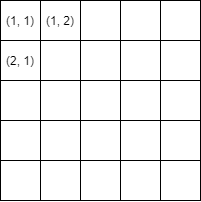
\includegraphics[clip,width=40mm]{a.png}
      \caption{Type A}
      \label{fig:a}
   	\end{center}
   \end{minipage}
   \begin{minipage}{0.33\hsize}
   	\begin{center}
      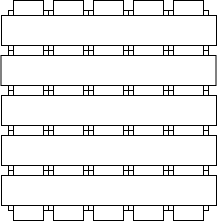
\includegraphics[clip,width=40mm]{b.png}
      \caption{Type B}
      \label{fig:b}
   	\end{center}
   \end{minipage}
   \begin{minipage}{0.33\hsize}
   	\begin{center}
      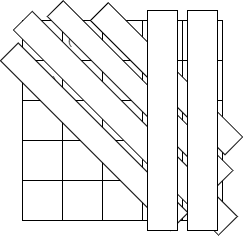
\includegraphics[clip,width=40mm]{c.png}
      \caption{Type C}
      \label{fig:c}
   	\end{center}
   \end{minipage}
  \end{figure*}

\section{今週やったこと}
\begin{itemize}
  \item $\alpha$の改良
\end{itemize}


\section{実験}

図 \ref{fig:a}, \ref{fig:b}, \ref{fig:c} に従来の$\alpha$の形式 A と
ベクトルの積で行列を作る タイプB, C のイメージを示した.

タイプB は学習する変数が少なく,
タイプC は縦方向の深さと斜め方向の接続距離の積で, 構造な特徴を反映できるようにした.

\begin{table}[tb]
  \begin{center}
    \caption{モデルの設定}
    \begin{tabular}{|c|c|} \hline
      base model & VGG19 \\ \hline
      Optim($w$) & SGD(lr=0.001, momentum=0.9) \\ \hline
      Optim($\alpha$) & Adam(lr=0.001, $\beta$=(0.5, 0.999)) \\ \hline
      Loss & Cross Entropy Loss \\ \hline
      dataset & cifar10 \\ \hline
      pretrain & true \\ \hline
      batch size & 64 \\ \hline
      train size & 25000 \\ \hline
      valid size & 25000 \\ \hline
    \end{tabular}
    \label{tab:setting}
  \end{center}
\end{table}

表 \ref{tab:setting}, にモデルの設定を示した.



\section{結果}

表 \ref{tab:result} に 3つのタイプのネットワーク性能と学習した 変数の数 を示した.
タイプ C は従来のタイプ A と比較して 0.09\% 向上した.
最も変数が少ない B よりも C がよりよい結果となった.
タイプ C の接続距離を考慮した構造がうまく作用したと思われる.

図 \ref{fig:a_r}, \ref{fig:b_r}, \ref{fig:c_r} に行列にしたときの
 $\alpha$ の重みを示した.
タイプA ではピンポイントな位置の推定ができている一方で,
タイプB, C は重みは直線上は似た値になっており, 大雑把な設定であったかもしれない.
それにも関わらず良い結果となったのは, 構造推定に関して主観的な拘束条件を加えたからであると考えられる.
しかし深さに対して $O(n^2)$ だった問題を解決する方法の1つは示せた.

\begin{table}[tb]
  \begin{center}
    \caption{結果}
    \begin{tabular}{|c|c|c|} \hline
      タイプ & accuracy(\%) & alpha \# \\ \hline\hline
      A & 93.71 & 17 * 17 \\ \hline
      B & 93.74 & 17 * 2 \\ \hline
      C & 93.80 & 17 * 3 - 1 \\ \hline
    \end{tabular}
    \label{tab:result}
  \end{center}
\end{table}

\begin{figure*}[tb]
 \begin{minipage}{0.33\hsize}
 	\begin{center}
    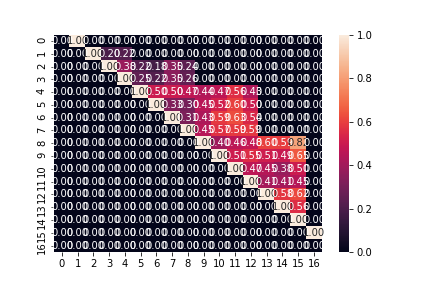
\includegraphics[clip,width=60mm]{al_a.png}
    \caption{Type A}
    \label{fig:a_r}
 	\end{center}
 \end{minipage}
 \begin{minipage}{0.33\hsize}
 	\begin{center}
    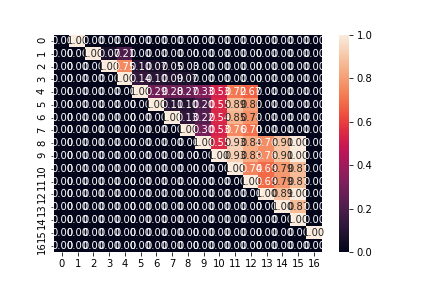
\includegraphics[clip,width=60mm]{al_b.png}
    \caption{Type B}
    \label{fig:b_r}
 	\end{center}
 \end{minipage}
 \begin{minipage}{0.33\hsize}
 	\begin{center}
    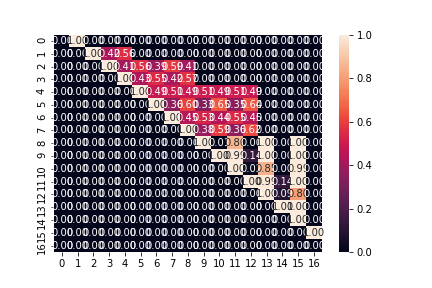
\includegraphics[clip,width=60mm]{al_c.png}
    \caption{Type C}
    \label{fig:c_r}
 	\end{center}
 \end{minipage}
\end{figure*}


% \begin{figure}[tb]
%   \begin{center}
%     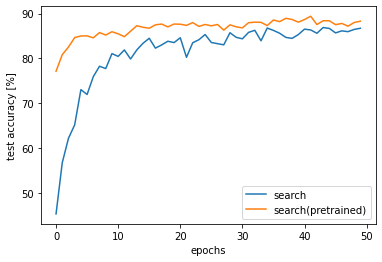
\includegraphics[clip,width=75mm]{acc.png}
%     \caption{世代ごとの test accuracy}
%     \label{fig:acc}
%   \end{center}
% \end{figure}


\section{今後の予定}
% なんとなくなんかの勉強をするとかではなく具体的に
\begin{itemize}
  \item 今回の3つの手法で TDGA の実験をする
\end{itemize}

% 参考文献リスト
\bibliographystyle{unsrt}
\bibliography{ref}
\end{document}
